\documentclass[addpoints]{exam}
%%%%%%%%%%%%%%%%%% PACKAGES %%%%%%%%%%%%%%%%%%%%%%%%
\usepackage{amsmath}
\usepackage{amsfonts}
\usepackage{tcolorbox}
\usepackage{tikz,tkz-euclide,tikz-3dplot}
%%%%%%%%%%%%%%%%%%%%%% MARGINS%% %%%%%%%%%%%%%%%%%%%
\extrawidth{.5in}
\extraheadheight{-.25in}
\extrafootheight{-.25in}
%%%%%%%%%%%%%%%%%% ANSWERS AND POINTS %%%%%%%%%%%%%%
%\printanswers
\pointsinrightmargin
\bracketedpoints
%%%%%%%%%%%%%%%%%% HEADER AND FOOTER %%%%%%%%%%%%%%%
\pagestyle{headandfoot}
\firstpageheadrule
\runningheadrule
\firstpageheader{\S3.EF Quiz}{}{AP Precalc\\Mr. Carey}
\runningheader{\S3.EF Quiz}{}{Mr. Carey}
\firstpagefooter{}{}{}
\runningfooter{ }{\thepage}{ }
%%%%%%%%%%%%%%%%%%%%%% NOTES %%%%%%%%%%%%%%%%%%%%%%%
%2025 - students did not begin calc section. Pacing too slow. Consider adding more problems to the review specifically involving verifying idents and solving equations.
%%%%%%%%%%%%%%%%%% DOCUMENT CONTENTS %%%%%%%%%%%%%%%
\begin{document}
\vspace{1in}

\noindent\makebox[.75\textwidth]{Name:\enspace\hrulefill} \hspace{.5in} Grade:\enspace\hrulefill/\numpoints

\vspace{.1in}

\begin{center}
    \fbox{\fbox{\parbox{5.5in}{\centering
    Answer the questions in the spaces provided on the following pages.  If you run out of room for an answer, continue on the back of the page. Show \textbf{all} your work to be able to receive full credit on any question.
    \textbf{YOU ARE A MISSILE}}}}
\end{center}

\section*{Part I - Formulas}

\noindent For each of the following questions, complete the specified trigonometric identity by filling in the blank(s).
\begin{questions}
\question[1] The Pythagorean Identity is \[\sin^2 x + \underline{\hspace{.75in}} = \underline{\hspace{.75in}}.\]

\vspace{\stretch{1}}

\question[1] The Power Reducing Identity for $\sin^2 x$ is \[\sin^2 x = \underline{\hspace{1.5in}}.\]

\vspace{\stretch{1}}    

\question[1] The Double Angle Identity for $\sin 2x$ is \[\sin 2x = \underline{\hspace{1.5in}}.\]

\vspace{\stretch{1}}

\question[1] The Angle Difference Identity for $\cos(x-y)$ is \[\cos(x-y) = \underline{\hspace{1.5in}}.\]

\vspace{\stretch{1}}

\question[1] The Angle Sum Identity for $\sin(x+y)$ is \[\sin(x+y) = \underline{\hspace{1.5in}}.\]

\vspace{\stretch{1}}
\end{questions}

\newpage
This page is intentionally left blank for printing purposes.

\phantom{hello world}
\vspace{\stretch{1}}

\newpage

\section*{Part II - No Calculator}

\begin{tcolorbox}[title=Recall: \textit{Fundamental Trigonometric Identities},title filled,colframe=black,sharpish corners,width=\linewidth]
    \begin{minipage}[t]{.45\linewidth}

        \begin{center}
            \textbf{Pythagorean Identities}
        \end{center}
        \[\sin^2\theta+\cos^2\theta=1\]
        \[\tan^2\theta+1=\sec^2\theta\]
        \[1+\cot^2\theta=\csc^2\theta\]
    \end{minipage}
    \hfil
    \begin{minipage}[t]{.45\linewidth}
        \begin{center}
            \textbf{Cofunction Identities}
        \end{center}
        \[\sin\left(\frac{\pi}{2}-\theta\right)=\cos\theta\]
        \[\cos\left(\frac{\pi}{2}-\theta\right)=\sin\theta\]
    \end{minipage}

    \vspace{.2in}

    \begin{minipage}[t]{.45\linewidth}
        \begin{center}
            \textbf{Sum and Difference Identities}
        \end{center}
        \[\sin(\alpha\pm\beta)=\sin\alpha\cos\beta\pm\cos\alpha\sin\beta\]
        \[\cos(\alpha\pm\beta)=\cos\alpha\cos\beta\mp\sin\alpha\sin\beta\]
    \end{minipage}
    \hfil
    \begin{minipage}[t]{.45\linewidth}
        \begin{center}
            \textbf{Even/Odd Identities}
        \end{center}
        \[\sin(-\theta)=-\sin\theta\]
        \[\cos(-\theta)=\cos\theta\]
        \[\tan(-\theta)=-\tan\theta\]
    \end{minipage}

    \vspace{.2in}

    \begin{minipage}[t]{.45\linewidth}
        \begin{center}
            \textbf{Double Angle Identities}
        \end{center}
        \[\sin(2\theta)=2\sin\theta\cos\theta\]
        \begin{align*}
            \cos(2\theta)&=\cos^2\theta-\sin^2\theta\\
            &=2\cos^2\theta-1\\
            &=1-2\sin^2\theta
        \end{align*}
        \[\tan(2\theta)=\frac{2\tan\theta}{1-\tan^2\theta}\]
    \end{minipage}
    \hfil
    \begin{minipage}[t]{.45\linewidth}
        \begin{center}
            \textbf{Power Reducing Identities}
        \end{center}
        \[\sin^2\theta=\frac{1-\cos2\theta}{2}\]
        \[\cos^2\theta=\frac{1+\cos2\theta}{2}\]
        \[\tan^2\theta=\frac{1-\cos2\theta}{1+\cos2\theta}\]
    \end{minipage}
\end{tcolorbox}

\begin{questions}
    \question[3] Plot the coordinate $\displaystyle\left(2,\frac{2\pi}{3}\right)$ and find two additional polar representations of this point with $-2\pi\leq\theta\leq2\pi$.
    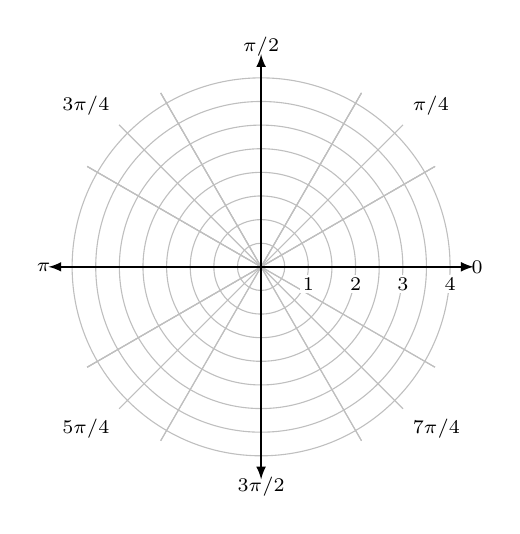
\begin{tikzpicture}[scale=.6]
        % Draw the lines at multiples of pi/6
        \foreach \ang in {0,...,31} {
            \draw [lightgray] (0,0) -- (\ang * 180 / 6:4.25);
        }
        % Add the labels at multiples of pi/4
        \foreach \ang/\lab/\dir in {
        0/0/right,
        1/{\pi/4}/{above right},
        2/{\pi/2}/above,
        3/{3\pi/4}/{above left},
        4/{\pi}/left,
        5/{5\pi/4}/{below left},
        7/{7\pi/4}/{below right},
        6/{3\pi/2}/below} {
        \draw [lightgray] (0,0) -- (\ang * 180 / 4:4.25);
        \node [fill=white] at (\ang * 180 / 4:4.25) [\dir] {\scriptsize $\lab$};
        }
        % Concentric circles and radius labels
        \foreach \s in  {1, 2, 3, 4} {
        \draw [lightgray] (0,0) circle (\s - 0.5);
        \draw [lightgray] (0,0) circle (\s);
        \node [fill=white] at (\s, 0) [below=1mm,inner sep=1pt] {\scriptsize $\s$};
        }
        \draw[latex-latex,semithick](-4.5,0)--(4.5,0);
        \draw[latex-latex,semithick](0,-4.5)--(0,4.5); 
        %\draw[domain=0:6.29,samples=200,smooth,-latex,thick,] plot ({deg(\x)}:{3*cos(\x r)});
    \end{tikzpicture}

    \vspace{\stretch{.2}}

    \question[2] Convert the rectangular coordiant $(4,4)$ to polar form.

    \vspace{\stretch{1}}

    \newpage

    \question[2] Convert $\displaystyle\left(-6,-\frac{7\pi}{6}\right)$ to rectangular form.

    \vspace{\stretch{1}}

    \question Convert the following rectangular equations to polar form. Leave your answer in the form $r=f(\theta)$. 
    \begin{parts}
        \part[3] $y^3=x^2$

        \vspace{\stretch{1}}

        \part[3] $2xy=5$

        \vspace{\stretch{1}}
    \end{parts}

    \newpage

    \question Convert the following polar equations to rectangular form. Leave your answer in the form $y=f(x)$ or the general form for the equation of a circle.
    \begin{parts}
        \part[3] $r=9\cos\theta$

        \vspace{\stretch{1}}

        \part[3] $\displaystyle\theta=\frac{11\pi}{6}$

        \vspace{\stretch{1}}

    \end{parts}


    \newpage

    

    \question[3] Given that $\tan u=\frac{3}{4}$ and $\sec v=-\frac{13}{5}$ with $0<u<\frac{\pi}{2}$ and $\sin v<0$, find the exact value of $\cos(u+v)$.

    \vspace{\stretch{.6}}

    \question Verify the following trigonometric identities.
    \begin{parts}
        \part[3] $\displaystyle2\sin\theta\cos\theta\sec2\theta=\tan2\theta$

        \vspace{\stretch{1}}

        \part[3] $\displaystyle\sin x\left(1-2\cos^2 x+\cos^4x\right)=\sin^5 x$

        \vspace{\stretch{1}}

    \end{parts}

    \newpage

    \question[5] Solve the following trigonometric equation \[\displaystyle\cos 4x+\sin2x=0.\] Find all solutions on the interval $0\leq x<2\pi$.

    \vspace{\stretch{1}}
    

    \question[4] Given the graph of a polar function, write the equation.
    \begin{parts}
        \begin{minipage}[t]{.45\linewidth}
            \part \phantom{hello}

            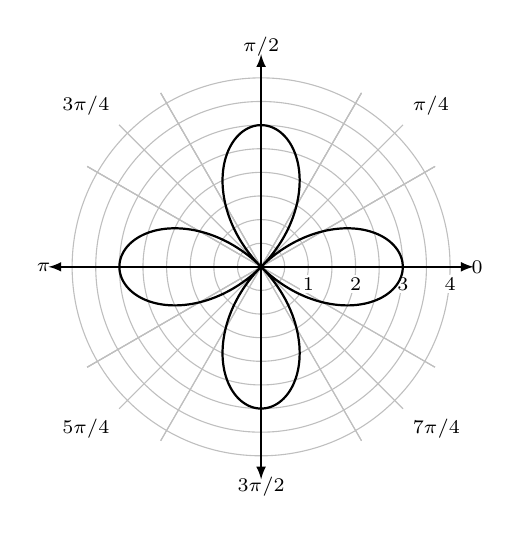
\begin{tikzpicture}[scale=.6]
             

                % Draw the lines at multiples of pi/6
                \foreach \ang in {0,...,31} {
                    \draw [lightgray] (0,0) -- (\ang * 180 / 6:4.25);
                }
                
                % Add the labels at multiples of pi/4
                \foreach \ang/\lab/\dir in {
                0/0/right,
                1/{\pi/4}/{above right},
                2/{\pi/2}/above,
                3/{3\pi/4}/{above left},
                4/{\pi}/left,
                5/{5\pi/4}/{below left},
                7/{7\pi/4}/{below right},
                6/{3\pi/2}/below} {
                \draw [lightgray] (0,0) -- (\ang * 180 / 4:4.25);
                \node [fill=white] at (\ang * 180 / 4:4.25) [\dir] {\scriptsize $\lab$};
                }
                
                % Concentric circles and radius labels
                \foreach \s in  {1, 2, 3, 4} {
                \draw [lightgray] (0,0) circle (\s - 0.5);
                \draw [lightgray] (0,0) circle (\s);
                \node [fill=white] at (\s, 0) [below=1mm,inner sep=1pt] {\scriptsize $\s$};
                }
    
                \draw[latex-latex,semithick](-4.5,0)--(4.5,0);
                \draw[latex-latex,semithick](0,-4.5)--(0,4.5); 
    
                \draw[domain=0:6.29,samples=200,smooth,-,thick,] plot ({deg(\x)}:{3*cos(2*(\x r))});
    
            \end{tikzpicture}
        \end{minipage}
        \hfill
        \begin{minipage}[t]{.45\linewidth}
            \part \phantom{hello}

            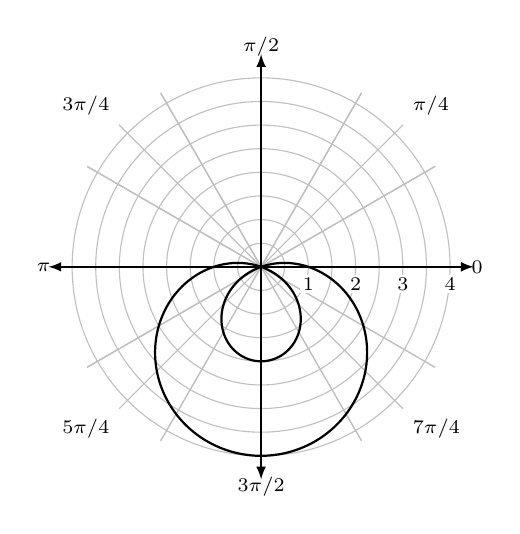
\begin{tikzpicture}[scale=.6]
                % Draw the lines at multiples of pi/6
                \foreach \ang in {0,...,31} {
                    \draw [lightgray] (0,0) -- (\ang * 180 / 6:4.25);
                }
                
                % Add the labels at multiples of pi/4
                \foreach \ang/\lab/\dir in {
                0/0/right,
                1/{\pi/4}/{above right},
                2/{\pi/2}/above,
                3/{3\pi/4}/{above left},
                4/{\pi}/left,
                5/{5\pi/4}/{below left},
                7/{7\pi/4}/{below right},
                6/{3\pi/2}/below} {
                \draw [lightgray] (0,0) -- (\ang * 180 / 4:4.25);
                \node [fill=white] at (\ang * 180 / 4:4.25) [\dir] {\scriptsize $\lab$};
                }
                
                % Concentric circles and radius labels
                \foreach \s in  {1, 2, 3, 4} {
                \draw [lightgray] (0,0) circle (\s - 0.5);
                \draw [lightgray] (0,0) circle (\s);
                \node [fill=white] at (\s, 0) [below=1mm,inner sep=1pt] {\scriptsize $\s$};
                }
    
                \draw[latex-latex,semithick](-4.5,0)--(4.5,0);
                \draw[latex-latex,semithick](0,-4.5)--(0,4.5); 
    
                \draw[domain=0:6.29,samples=200,smooth,-,thick,] plot ({deg(\x)}:{1-3*sin(\x r)});
    
            \end{tikzpicture}
        \end{minipage}

        \vspace{\stretch{.2}}
    \end{parts}


\newpage

\question[5] On the polar axes below, graph the function $r=-2\sin3\theta$ for $0\leq\theta\leq2\pi$. Then, specify what lines of symmetry the curve has.

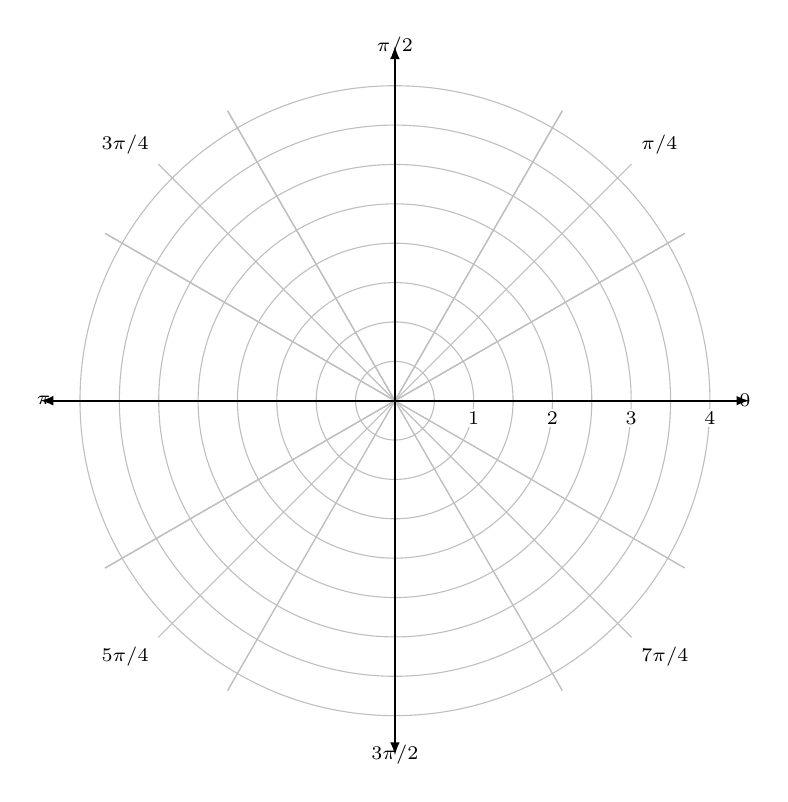
\begin{tikzpicture}[scale=1]
    % Draw the lines at multiples of pi/6
    \foreach \ang in {0,...,31} {
        \draw [lightgray] (0,0) -- (\ang * 180 / 6:4.25);
    }
    
    % Add the labels at multiples of pi/4
    \foreach \ang/\lab/\dir in {
    0/0/right,
    1/{\pi/4}/{above right},
    2/{\pi/2}/above,
    3/{3\pi/4}/{above left},
    4/{\pi}/left,
    5/{5\pi/4}/{below left},
    7/{7\pi/4}/{below right},
    6/{3\pi/2}/below} {
    \draw [lightgray] (0,0) -- (\ang * 180 / 4:4.25);
    \node [fill=white] at (\ang * 180 / 4:4.25) [\dir] {\scriptsize $\lab$};
    }
    
    % Concentric circles and radius labels
    \foreach \s in  {1, 2, 3, 4} {
    \draw [lightgray] (0,0) circle (\s - 0.5);
    \draw [lightgray] (0,0) circle (\s);
    \node [fill=white] at (\s, 0) [below=1mm,inner sep=1pt] {\scriptsize $\s$};
    }

    \draw[latex-latex,semithick](-4.5,0)--(4.5,0);
    \draw[latex-latex,semithick](0,-4.5)--(0,4.5); 

    %\draw[domain=0:6.29,samples=200,smooth,-,thick,] plot ({deg(\x)}:{1-3*sin(\x r)});

\end{tikzpicture}



\end{questions} 



\newpage

\section*{Part III - Calculator Allowed}

\begin{questions}
\question[2] Consider the graph of $f(\theta)=1+2\sin\theta$ for $0\leq\theta\leq2\pi$. Which of the following statements is true about the distance between $f(\theta)$ and the origin?
\begin{choices}
    \choice The distance is increasing on $0\le\theta\le\frac{\pi}{2}$, becuase $f(\theta)$ is positive and increasing on the interval.
    \choice The distance is increasing on $\frac{3\pi}{2}\le\theta\le\frac{11\pi}{6}$, becuase $f(\theta)$ is negative and increasing on the interval.
    \choice The distance is decreasing on $0\le\theta\le\frac{\pi}{2}$, becuase $f(\theta)$ is positive and decreasing on the interval.
    \choice The distance is decreasing on $\frac{3\pi}{2}\le\theta\le\frac{11\pi}{6}$, becuase $f(\theta)$ is negative and decreasing on the interval.    
\end{choices}

\vspace{\stretch{.5}}

\question[2]  What is the average rate of change of the polar curve $r=2+4\cos\theta$ on the interval $\displaystyle\left[0,\frac{\pi}{2}\right]$?

\vspace{\stretch{1}}

\newpage

\question Consider the function $f(\theta)=-2+1\sin\theta$ for $0\leq\theta\leq2\pi$.
\begin{parts}
    \part[2] On the inteval when $\theta=0$ to $\theta=\frac{\pi}{6}$, is $r=f(\theta)$ increasing, decreasing, or neither? How do you know?
    
    \vspace{\stretch{1}}

    \part[2] On the interval $\left[\frac{\pi}{2},\frac{2\pi}{3}\right]$, is the distance between $f(\theta)$ and the origin increasing or decreasing? Justify your answer.

    \vspace{\stretch{1}}
\end{parts} 




\end{questions}





\end{document}